This section describes the relationships between the different classes
described in \cref{sub:pd_classes}. These relationships will be
visualised in a class diagram as described
in~\cite{mathiassen2001objektorienteret}.

The authors of~\cite{mathiassen2001objektorienteret} operate with three
main structuring techniques.

\begin{description}
\item[Generalisation] Generalisation is used to describe a \enquote{is-a}
  relationship between classes. A class is called a
  superclass when another class inherits attributes and operations
  from this superclass. The other class is now a subclass of the
  superclass. In class diagrams, generalisation is denoted by a
  triangular arrow pointing from the subclass to the superclass.
\item[Aggregation] Aggregation is used to describe a
  \enquote{contains} relationship between classes. In class diagrams,
  aggregation is denoted by a rhombus shaped arrow.
\item[Association] Association is used to describe that two classes
  are aware of each other. Association is denoted in class diagrams by
  a line between each class.
\end{description} \chnote{Hvorfor er det beskrevet?}

Based on these structuring techniques, a class diagram showing the structure of the classes in the problem domain of the system has been made. See \cref{fig:pd_structure}. Every \enquote{User} class has an association with either zero or one \enquote{Track} classes, i.e. they have voted on a track. A \enquote{Track} can have an association with an \enquote{Audio system} class in that it is currently being played. The \enquote{Playlist} class contains zero or more \enquote{Track} classes, i.e. the tracks yet to be played. A \enquote{Playlist} class has an association with a \enquote{Filter}, i.e. the playlist is filtered by a filter.

\begin{figure}
  \centering
  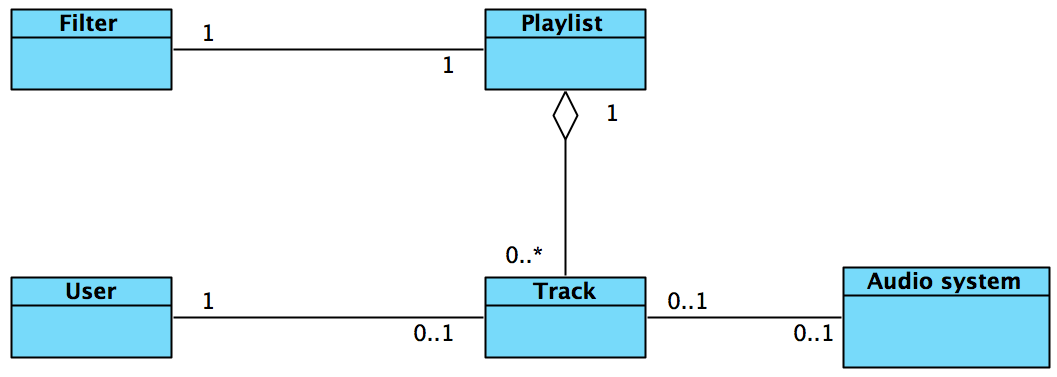
\includegraphics[width=\textwidth]{pd_structure.png}
  \caption{Class diagram of problem domain}\label{fig:pd_structure}
\end{figure}
